\chapter{Une piste de solution: l'augmentation de la natalité}
\paragraph{}Dans le premier chapitre nous avons vu que le taux de natalité oscille entre 1,5 et 1,7 en moyenne dans l’Europe des 28 aux cours des quinze dernière année, alors que le seuil de renouvellement ce situe autour de 2,1\citep{eur-lex}. Si la population européenne continue de croître c’est donc uniquement dû à l’immigration.  La première question à ce poser est de savoir si l’augmentation du taux de natalité pourrait être une solution contre le vieillissement de la population et si oui dans quelle mesure ce taux de natalité devrait-il augmenter . Finalement, quelle mesure pourrait-on pendre pour que le taux de natalité augmente car il est évident que ce n’est pas quelque chose que l’ont peut imposer. 
\section{L'augmentation de la natalité une vraie solution ?}
\paragraph{}L’article de Héran\citep[pp.1]{heran} répond à la première partie de la question lorsqu’il parle d’une part évitable et d’une part inévitable du vieillissement de la population. La part inévitable est dû au baby boom et à l’accroissement de la durée de vie. La part évitable est le vieillissement par le bas qui peut être ralenti. L’article Héran\citep[pp.5-6]{heran} détails pour chaque pays de l’Europe l’évolution des jeunes (0-14 ans), de la population active (15-64 ans) et des personnes agées (+65 ans), nous n’avons repris dans le graphe \ref{vieillissement} que la France et l’Allemagne car ces deux pays représente respectivement un taux de natalité très élevé (2,01) et très faible (1,42) par rapport à la moyenne Européenne.  Et l’un comme l’autre voit leur population de personnes âgées augmenter de 80\%. Cela représente la part inévitable du vieillissement. Part contre on peut observer une diminution de 20\% du reste de la population en Allemagne alors que celle-ci reste stable en France. 

\begin{figure}[h!]
    \begin{center}
        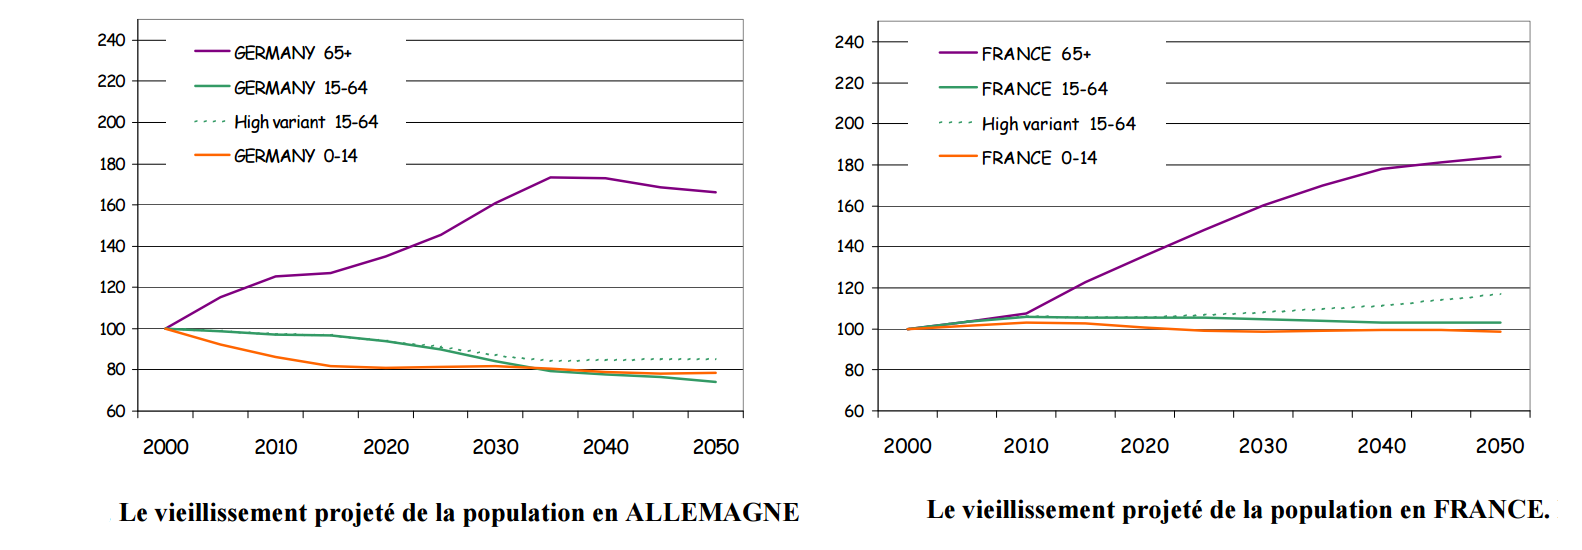
\includegraphics[scale=0.4]{document/vieillissement.png}
        \caption{Source: Héran\citep[pp.5-6]{heran}}
        \label{vieillissement}
    \end{center}
\end{figure}

Les graphes \ref{FR-DE_natalite.png} montre les projections d’Eurostat\citep{eurostat_europop13} pour les deux pays jusqu’en 2080. Le premier représente le scénario sans immigration. Dans ce scénario, on peut observer que malgré une augmentation du taux de natalité à 1,7, l’Allemgane perd 30 millions d’habitants alors que la France croît d’abord légèrement pour se stabiliser vers 70 millions. Le scénario moyen retenu par Eurostat\citep{eurostat_europop13} ne fait qu’atténuer la perde d’habitant pour l’Allemagne alors que la France gagne presque 15 Millions d’habitants. Est-ce que l’augmentation de la natalité est une solution aux vieillissement de la population ? Non, elle ne pourra pas contrecarré les effets du baby boom et de l’augmentation de l’espérance de vie mais elle reste indispensable sur le long terme pour le maintient de la population à son niveau actuelle car l’immigration à elle seule ne permettra pas le maintien de la population. Si le taux se situe proche du seuil de remplacement, la pyramide des âges finira pas s'équilibrer et à ressembler à un cylindre une fois l’effet du Baby Boom passer après 2050. L’augmentation doit se maintenir dans le temps et ne plus redescendre, sinon nous pourrions nous retrouver en fasse d’un nouvel effet Baby Boom. 

\begin{figure}[h!]
    \begin{center}
        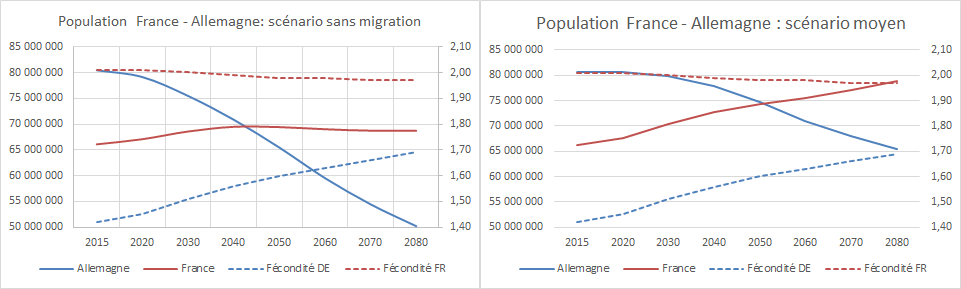
\includegraphics[scale=0.6]{document/FR-DE_natalite.png}
        \caption{Source: Eurostat\citep{eurostat_europop13}}
        \label{FR-DE_natalite.png}
    \end{center}
\end{figure}

\section{Les causes d'un faible taux de natalité}
\paragraph{}Il faut ensuite se demander pourquoi le taux de natalité est faible dans des pays comme l’Allemagne ou les pays du sud (Espagne, Italie, Portugal)\citep{4model}  et quelle politique pourrait favoriser une augmentation. 

\paragraph{}Pour Le Bras, la raison économique qui explique ces différences est sans doute la plus simple, la difficulté à accéder à un emploi à pour effet de diminuer la fécondité\citep[pp.25]{heran} car les femmes repartissent leur efforts entre emploi et famille et si trouver ou maintenir un emploi nécessite beaucoup d’effort il ne reste plus d’énergie à consacrer à la famille et étonnamment, on remarque dans les pays plus traditionnel comme l’Espagne, le Portugal ou l’Italie, le fait d’avoir une femme maintenu au foyer diminue la fécondité. Il a pu établir une corrélation entre la fécondité et le taux d'activité des femmes. 

\paragraph{}L’Allemagne est malgré tout une exception. Elle est dû à une mentalité très rigide en matière de famille où la mère doit prendre en charge les enfants fait que celle-ci culpabilise si elle doit continuer à travailler. Il y a d’ailleurs un terme pour ces femmes en Allemagne RabenMutter\citep{mutter}. 

\paragraph{}Le rapport Roy\citep{quebec} décrit les trois conditions nécessaires à la venue d’un enfant au sein d’un couple : la sécurité financière, une relation stable et sûr, un conjoint qui partage les tâches ménagères\citep[pp.19]{quebec}. Il expose aussi plusieurs théorie du faible taux de fécondité. La première, la théorie du choix rationnel considère la mise en balance des coûts directs et indirects\footnote{Parmis les coût indirecte, on peut citer le fait de devoir quitter son travail ou de travailler à mi-temps, la mise en pause de la carrière} de l’enfant d’un coté et l’avantage psychologique de l’autre. Si il est possible de faire peser plus l’avantage psychologique en influençant les mentalités, il est plus facile de diminuer le poids des coût directe et indirecte lié aux enfants\citep[pp.23]{quebec}. La seconde est celle de l’évitement du risque, selon cette théorie les coût associé au fait d’avoir des enfants est certain mais les bénéfices qu’on va en tirer ne sont que hypothétiques et si son avenir personnel est incertain, les personnes vont se tourner vers le choix le moins risquer: l’absence d’enfant\citep[pp.24]{quebec}. Une troisième est celle de l’équité des sexe\citep[pp.25]{quebec}. Cette théorie distingue l’équité des sexes au travail et à la maison. Si celles-ci ne sont pas en adéquation, la participation à la vie active accumulé avec l'ensemble des tâches ménagères serait un poids trop lourd pour envisager la maternité. 
\section{Les politiques possibles pour encourager la natalité}
Au vue de ces théories, il apparaît plus clairement quelles politiques pourraient favoriser une augmentation de la natalité. Une politique familiale doit être mise en place plutôt qu’une politique nataliste qui est mal perçu en Europe dû au poids de l’histoire\citep[pp.27]{quebec}\footnote{Cela pourrait, par exemple, rappeler des politiques comme celle utilisée par lé régime Nazi où la femme à pour seul objectif d'enfanter\citep{nazi}}. L’objectif de cette politique serait de lever les obstacles à la décision d’avoir un enfant. Elle devrait selon Roy\citep[pp.43-46]{quebec}:


\begin{itemize}
  \item favoriser l’emploi car comme nous l’avons vu la facilité à l’accès à un emploi pour les femmes favorise la fécondité et l’emploi reste le meilleur facteur de stabilité financière. 
  \item favoriser la conciliation du travail et de la famille, qui pourrait se concrétiser sous la forme des mesures suivantes : congé parentaux, l’accueil des enfants dés la fin des congés parentaux, permettre des horaires de travail plus souple, favorisé l’égalité des sexes au travail. 
  \item compenser les coûts générer par un enfant car ceux-ci représente le meilleur investissement pour une société et la famille permet la naissance de cette investissement, un service qui devrait être rémunéré. Parmi ces mesures, on peut citer des allocations familiales, les allocations pour la scolarité, des avantages fiscaux pour les parents et des services gratuits pour les familles.
  \item favoriser un changement de mentalité, absolument nécessaire en Allemagne, favoriser les attitudes positives envers les enfants et les parents, promouvoir une égalité des sexes aux travail mais aussi à la maison. 
\end{itemize}

Pour finir, selon Héran, il est important que les mesures prises en faveur de la famille soient inscrites dans la durée et subsistent aux alternances politique car les futurs parents doivent pouvoir bénéficier d’une politique stable tout au long du développement de leur enfants\citep[pp.14]{heran}. 

Malgré cela, la conclusion de Le Bras n’est pas très optimiste: “Il faut renoncer à l’idée d’assister rapidement à une reprise de la fécondité en Europe”\citep[pp.27]{heran} car pour lui deux modèles de fécondité se partage l’Europe, un modèle basé sur l’intervention de l’état dans les pays du nord et en France et un modèle centré sur le rôle de la famille et les mesures qui favorisent la fécondité ne serait pas la raison de ces deux modèles mais la conséquences. S’il est relativement facile de changer les politiques familiale il l’est beaucoup plus de changer les mentalités ancrée dans une société. “La France a mis cent ans à tirer le bénéfice de sa législation natalise.”\citep[pp.28]{heran}

Nous avons vu que l’augmentation de la natalité permettrait un maintien de la population en Europe à long terme et allié à une immigration constante conduirait à un accroissement de la population et à une stabilisation de l'âge moyen de la population. Mais il faut se rendre à l’évidence, ces approches n'apportera aucune solution à cours terme, elle doit donc être combiné à d’autre solutions.  

